\documentclass[10pt, oneside, pdftex]{article}
\usepackage{amsmath, amstext, amsfonts, amssymb}
\usepackage[pdftex]{graphicx}
\usepackage{subfigure, longtable}
\usepackage{float}
\usepackage{rotating}
\usepackage{longtable}
\usepackage{url}
\usepackage{setspace}
\usepackage{pdflscape}
\usepackage{threeparttable}
\usepackage[left=2.54cm,bottom=2.00cm,top=2.00cm,right=2.54cm]{geometry}
%%%%%%%%%%%%%%%%%%%%%%%%%%%%%%%%%%%%%%%%%%%%%%%%%%%
%% Fonts in Document
%%%%%%%%%%%%%%%%%%%%%%%%%%%%%%%%%%%%%%%%%%%%%%%%%%%
%\usepackage{times}
%\usepackage{pslatex}
%\usepackage{newcent}
%\usepackage{palatcm}
%\usepackage{palatino}
%\usepackage[T1]{fontenc}
\usepackage[scaled]{helvet}
\renewcommand*\familydefault{\sfdefault}
%\renewcommand*{\encodingdefault}{T1}

%%%%%%%%%%%%%%%%%%%%%%%%%%%%%%%%%%%%%%%%%%%%%%%%%%%
% Here begins the document
%%%%%%%%%%%%%%%%%%%%%%%%%%%%%%%%%%%%%%%%%%%%%%%%%%%
\begin{document}
\title{RNA Motifs}
\author{Mauricio Esguerra}
\maketitle

As mentioned in  Chapter 2 the most common  perspectives for RNA motif
recognition  and  discovery are  the  atom  and  bond based  ones, the
rigid-body-based perspective has been  rather unexplored. The two main
questions that we would like to answer in this context are:

\begin{enumerate}
\item{Can  the geometric rigid-block  description of  base-pairing and
  base-stacking solve the problem of defining RNA structural motifs?}
\item{Can we use quantities derived  from the 3DNA software package to
  make and automatic  search for a known motif,  for example, the GNRA
  tetraloop motif, and perhaps find unknown motifs?}
\end{enumerate}

We have  started with  the second  question and have  chosen as
workhorse the well known GNRA tetraloop motif. We have also used other
quantities  (e.g.  endocyclic  and  exocyclic base-overlaps)  obtained
with  the 3DNA  \cite{lu2003, lu2008b}  package, and  quantified their
relationship to RNA motifs.

\section{The GNRA Tetraloop}

Description and brief survey of the motif.
First  formally  described  by  Woese \cite{woese1990}  in  1990  from
comparative  sequence analysis,  although supossedly  recognized since
1985. First characterized in NMR by Heus and Pardi \cite{heus1991}





\centering 
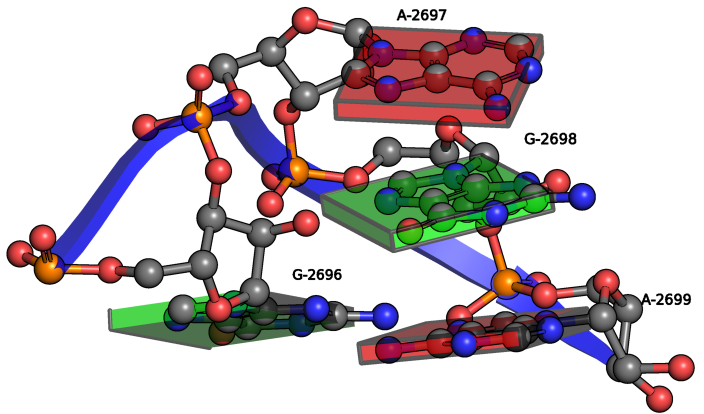
\includegraphics[angle=0, scale=0.5]{gnra.png}
\caption{GNRA   Tetraloop  from   \textit{Thermus   Thermophilus}  23S
  Ribosomal RNA PDB-ID:1ffk.}
\end{figure}


In the  RNA ontology consortium (ROC)  meeting of May,  2009 a reduced
dataset        of        RNA        structures        found        at:
\url{https://docs.google.com/Doc?id=dhrmkfmn_13ftpbjcgq}    was   made
available to participants with the  purpose of allowing them to search
for RNA motifs, which would later be compared between groups.





%\section{Canonical "Noise"}
%To be able to say anything about motifs it's crucial to get rid of the
%"noise" which is given by the canonical base-pair steps.
%One would think that perhaps  the X3DNA-Parser of Dr. Yurong Xin could
%help  in the  task, but  then, it  can't, because  it's based  on what
%base-pairs  have  been found,  therefore,  it  tells  me about  single
%stranded interactions,  it doesn't tell  me about bases which  are not
%forming interactions and are alone.

%\subsection{3DNA-Parser}
%We started by using Dr. Yurong Xin's 3DNA-Parser hoping that the
%description of the enclosing base pair in the loop, that is, the
%sheared G$\cdot$A, would have a characteristic signature.
%We found that such is not the case. We know from Major et
%al. \cite{lemieux2006} that there should be at least 21 GNRA tetraloops
%in the 23S subunit of rRNA. We used the G2696 N2697 R2698 A2699
%tetraloop as a seed (as can be seen in Figure 1.1) and found out
%that according to Dr. Xin's helical classification the enclosing G is
%classified as $S_{hq}$ and A is classified as $H_{e}$. 

%We then searched all such instances for G$\cdot$A base-pairs and we found seven hits,
%but none were in fact GNRA tetraloops.

\subsection{Overlap Scores} 
We clustered the overlap values impossing a cutoff of values
of [1-8]. Since a large amount of overlap values are exactly zero (33\%), so,
without the cutoff the zero values "overshadow" the data.
\begin{figure}[htbp]
\centering 
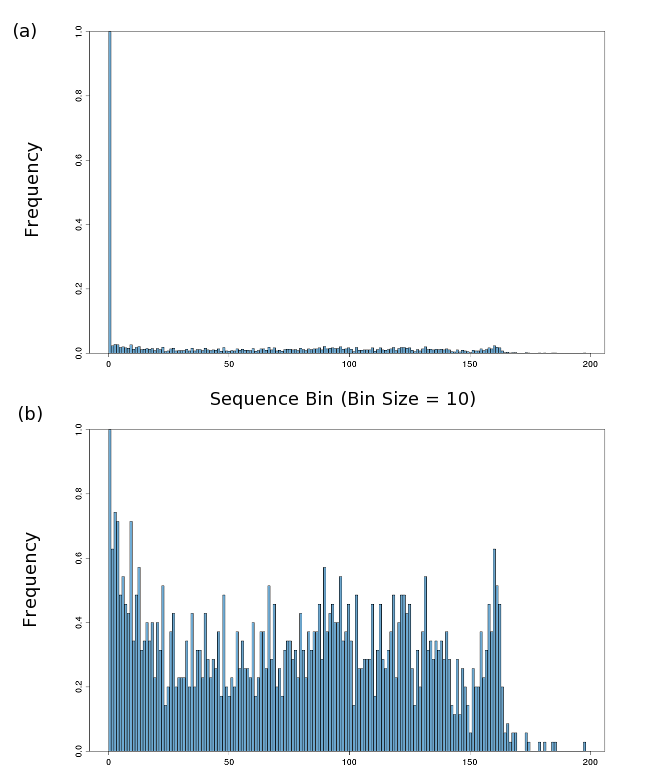
\includegraphics[angle=0, scale=0.8]{histocompare.png}
\caption{Normalized histograms showing the distribution of overlap values in 
the 23S subunit or \textit{Thermus Thermophilus} rRNA, PDB-ID:1jjk. In histogram 
(a) all values are included, but in histogram (b) only values greater than zero are 
included. Notice the high preponderance of zero values, exactly 897 out of a total
of 2705.}
\end{figure}
For this case we obtained a ``good'' dendrogram as seen in Figure 1.2.
\begin{figure}[htbp]
\centering 
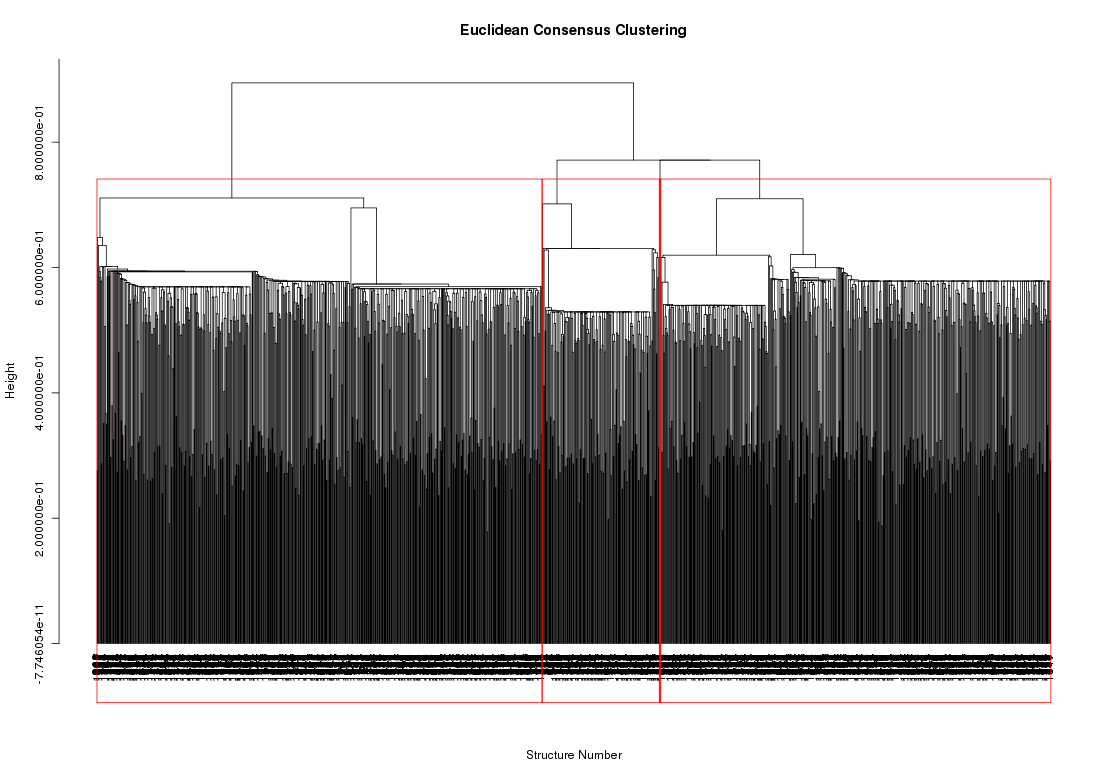
\includegraphics[angle=90, scale=0.6]{eucli_cons.png}
\caption{Dendrogram for consensus clustering of overlap scores in the ribosome.
Zero values filtered out and remaining data normalized.}
\end{figure}

The next step in this analysis will be to find the structures which
correspond to this clusters and superimpose and align them using
Kabsh's algorithm to be able to determine their RMSD's.

Many people start their RNA Motif identification and classification
algorithms by splitting RNA structures into what is helical and what
is not, and then finding interactions between these two groups. We
believe that we could do a similar exercise with 3DNA by using the scalar
product of helical axis vectors and once helical and non-helical regions are found we might be able to use 3DNA Parser to look for characteristic interactions.

%\section{Triplets on RNA (comparison to Laing et al.)}

\begin{equation}
    \label{simple_equation}
    \alpha = \sqrt{ \beta }
\end{equation}

\subsection{Subsection Heading Here}
Write your subsection text here.

\bibliographystyle{plain}
\bibliography{biblio}	
\end{document}
